\documentclass[letterpaper,10pt]{article}
\usepackage[utf8]{inputenc}
\usepackage{fullpage}
\usepackage[english]{babel}
\usepackage{amsmath}
\usepackage{caption}
\usepackage{subcaption}
\usepackage{graphicx}

\renewcommand{\arraystretch}{1.4}
\setlength{\parindent}{0cm}

\begin{document}

\noindent
\begin{flushright}
    \large\textbf{Miguel Alcón Doganoc} \\
    Combinatorial Problem Solving \\
    May 7, 2019
\end{flushright}

\noindent
{\huge{\textbf{Logic Synthesis}}}

\section{Variables}
Given the number of input signals $n$, the depth $d$, and the specification (truth table) of the logical circuit, I defined the following variables:
\begin{itemize}
    \item $\mathbf{c_{i,j}}:=$ ``Code of the node ($i$,$j$)'', where
    \begin{itemize}
        \item $i \in \{0,1,...,d\}$
        \item $j \in \{0,1,...,2^i-1\}$
    \end{itemize}
    \item $\mathbf{b_{i,j}^{(t)}}:=$ ``Boolean value of the node ($i,j$) for the row $t$ of the truth table'', where
    \begin{itemize}
        \item $i \in \{0,1,...,d\}$
        \item $j \in \{0,1,...,2^i-2\}$
        \item $t \in \{0,1,...,2^n-1\}$
    \end{itemize}
\end{itemize}

For example, for a NOR-circuit that implements the functionality of an AND gate (see figure \ref{fig:original}), with $n = d = 2$, one possible solution for the variables $c_{i,j}$ and $b_{i,j}^{(0)}$, with $i \in \{0,1,...,6\}$, is shown in figures \ref{subfig:ci} and \ref{subfig:bit}, respectively.
\begin{figure}[hbtp]
    \centering
    \begin{subfigure}[b]{0.45\textwidth}
        \raisebox{18mm}{\begin{tabular}{c c | c | c}
            $x_1$ & $x_2$ & $y$ & $t$\\ \hline
            0 & 0 & 0 & 0 \\
            0 & 1 & 0 & 1 \\
            1 & 0 & 0 & 2 \\
            1 & 1 & 1 & 3 \\
        \end{tabular}}
    \end{subfigure}\hspace{-0.2\textwidth}
    \begin{subfigure}[b]{0.45\textwidth}
        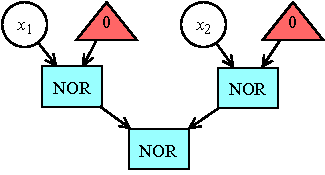
\includegraphics[width=\textwidth]{circuit.pdf}
    \end{subfigure}
    \caption{Truth table of $y$ = AND($x_1,x_2$) and NOR-circuit implementing it.}
    \label{fig:original}
\end{figure}

\begin{figure}[hbtp]
    \centering
    \begin{subfigure}[b]{0.30\textwidth}
        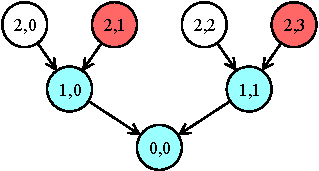
\includegraphics[width=\textwidth]{i.pdf}
        \caption{$i$}
        \label{subfig:i}
    \end{subfigure}
    \hspace{0.01\textwidth}
    \begin{subfigure}[b]{0.30\textwidth}
        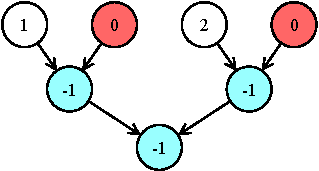
\includegraphics[width=\textwidth]{ci.pdf}
        \caption{$c_{i,j}$}
        \label{subfig:ci}
    \end{subfigure}
    \hspace{0.01\textwidth}
    \begin{subfigure}[b]{0.30\textwidth}
        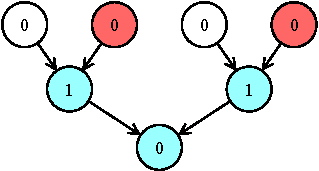
\includegraphics[width=\textwidth]{bit.pdf}
        \caption{$b_{i,j}^{(0)}$}
        \label{subfig:bit}
    \end{subfigure}
    \caption{Visual representation of ($i,j$) and both variables.}
    \label{fig:variables}
\end{figure}


\section{Constraints}
In order to simplify the definition of the constraints, I define three functions. Given the variable $v_{i,j}$, with $v_{i,j} = c_{i,j}$ or $b_{i,j}^{(t)}$,
\begin{itemize}
    \item \textbf{left($v_{i,j}$)} := ``Variable corresponding to the one on the left of $v_{i,j}$''
    \item \textbf{right($v_{i,j}$)} := ``Variable corresponding to the one on the right of $v_{i,j}$''
    \item \textbf{bit-up(k,t)} := ``Boolean value of $x_k$ in the $t$ row of the truth table''
\end{itemize}

So, the constraints are the following:
\begin{enumerate}
    \item $c_{d,j} \geq 0$
    \item $c_{i,j} \geq 0 \Rightarrow (\mathbf{left}(c_{i,j}) = 0 \land \mathbf{right}(c_{i,j}) = 0)$
    \item $c_{i,j} = -1 \Rightarrow (\mathbf{left}(c_{i,j}) \geq \mathbf{right}(c_{i,j}))$
    \item $(c_{i,j} = -1 \land (\mathbf{left}(c_{i,j}) > 0 \lor \mathbf{right}(c_{i,j}) > 0)) \Rightarrow (\mathbf{left}(c_{i,j}) \geq \mathbf{right}(c_{i,j}))$
    \item $c_{i,j} = -1 \Rightarrow (b_{i,j}^{(t)} = \lnot (\mathbf{left}(b_{i,j}^{(t)}) \lor \mathbf{right}(b_{i,j}^{(t)})))$
    \item $c_{i,j} = 0 \Rightarrow \lnot b_{i,j}^{(t)}$
    \item $c_{i,j} = k \Rightarrow b_{i,j}^{(t)}$
    \item $c_{i,j} = k \Rightarrow \lnot b_{i,j}^{(t)}$
\end{enumerate}


\end{document}